
\section{Simulations}\label{sec-sim}


To assess the finite sample performance of our methods, we conduct a number of simulations. In Sections \ref{subsec-sim-1} and \ref{subsec-sim-2}, we investigate the performance of our multiscale test and compare it to the SiZer methods for time series developed in \cite{Rondonotti2004} and \cite{Rondonotti2007}. In Section \ref{subsec-sim-3}, we analyse the finite sample properties of our long-run variance estimator from Section \ref{subsec-error-var-AR} and compare it to the estimator of \cite{Hall2003}. 


\subsection{Size and power properties of the multiscale test}\label{subsec-sim-1} 


Our simulation design mimics the situation in the application example of Section \ref{sec-data}. We generate data from the model $Y_{t,T} = m(t/T) + \varepsilon_t$ for different trend functions $m$, error processes $\{\varepsilon_t\}$ and time series lengths $T$. The error terms are supposed to have the AR($1$) structure $\varepsilon_t = a_1 \varepsilon_{t-1} + \eta_t$, where $a_1 \in \{-0.5,-0.25,0.25,0.5\}$ and $\eta_t$ are i.i.d.\ standard normal. In addition, we consider the AR($2$) specification $\varepsilon_t = a_1 \varepsilon_{t-1} + a_2 \varepsilon_{t-2} + \eta_t$, where $\eta_t$ are normally distributed with $\ex[\eta_t] = 0$ and $\ex[\eta_t^2] = \nu^2$. We set $a_1 = 0.167$, $a_2 = 0.184$ and $\nu^2 = 0.322$, thus matching the estimated values obtained in the application of Section \ref{sec-data}. To simulate data under the null hypothesis, we let $m$ be a constant function. In particular, we set $m = 0$ without loss of generality. To generate data under the alternative, we consider the trend functions $m(u) = \beta (u - 0.5) \cdot \ind(0.5 \le u \le 1)$ with $\beta = 1.5,2.0,2.5$. These functions are broken lines with a kink at $u = 0.5$ and different slopes $\beta$. Their shape roughly resembles the trend estimates in the application of Section \ref{sec-data}. The slope parameter $\beta$ corresponds to a trend with the value $m(1) = 0.5 \beta$ at the right endpoint $u = 1$. We thus consider broken lines with the values $m(1) = 0.75, 1.0, 1.25$. Inspecting the middle panel of Figure \ref{plot-results-app1}, the broken lines with the endpoints $m(1) = 1.0$ and $m(1) = 1.25$ (that is, with $\beta = 2.0$ and $\beta = 2.5$) can be seen to resemble the local linear trend estimates in the real-data example the most (where we neglect the nonlinearities of the local linear fits at the beginning of the observation period). The broken line with $\beta = 1.5$ is closer to the null, making it harder for our test to detect this alternative.\footnote{The broken lines $m$ are obviously non-differentiable at the kink point. We could replace them by slightly smoothed versions to satisfy the differentiability assumption that is imposed in the theoretical part of the paper. However, as this leaves the simulation results essentially unchanged but only creates additional notation, we stick to the broken lines.}


%To simulate data under the null, we let $m$ be a constant function. In parti\-cular, we set $m = 0$ without loss of generality. To generate data under the alternative, we consider trend functions of the form $m(u) = \beta \cdot (u - 0.5) \cdot \ind(0.5 \le u \le 1)$ with the slope parameter $\beta$. These functions are broken lines with a kink at $u = 0.5$. Their shape roughly resembles the trend estimates in the application of Section \ref{sec-data}. For each AR specification of the errors, we consider three different slopes $\beta = s_\beta \cdot \sigma$ with $s_\beta \in \{1.7,2.3,2.9\}$ and $\sigma^2$ being the long-run error variance. The parameter $s_\beta$ is closely related to the signal-to-noise ratio in the model $Y_{t,T} = m(t/T) + \varepsilon_t$: The larger $s_\beta$, the stronger is the trend $m$ compared to the long-run error variance $\sigma^2$. The values $s_\beta \in \{ 1.7, 2.3, 2.9\}$ are motivated by the application example in Section \ref{sec-data}: For the AR($2$) specification which mimics the data example, it holds that $\beta \approx 1.5, 2.0, 2.5$ for $s_\beta = 1.7,2.3,2.9$. As the slope parameter $\beta$ corresponds to a trend with the value $m(1) = 0.5 \cdot \beta$ at the right endpoint $u = 1$, we thus consider broken lines with the values $m(1) \approx 0.75, 1.0, 1.25$ in this case. Inspecting the middle panel of Figure \ref{plot-results-app1}, the broken lines with the endpoints $m(1) \approx 1.0$ and $m(1) \approx 1.25$ (that is, with $s_\beta = 2.3$ and $s_\beta = 2.9$) can be seen to resemble the local linear trend estimates in the real-data example the most (where we neglect the nonlinearities of the local linear fits at the beginning of the observation period). The broken line with $s_\beta = 1.7$ has a smaller slope $\beta$ and is thus closer to the null, making it harder for our test to detect this alternative.\footnote{The broken lines $m$ are obviously non-differentiable at the kink point. We could replace them by slightly smoothed versions to satisfy the differentiability assumption that is imposed in the theoretical part of the paper. However, as this leaves the simulation results essentially unchanged but only creates additional notation, we stick to the broken lines.}


\begin{sidewaystable}
\centering
\footnotesize{
\caption{Size of our multiscale test for different AR parameters $a_1$ and $a_2$, sample sizes $T$ and nominal sizes $\alpha$.}\label{tab:size_test}
\newcolumntype{C}[1]{>{\hsize=#1\hsize\centering\arraybackslash}X}
\newcolumntype{Z}{>{\centering\arraybackslash}X}
\begin{tabularx}{\textwidth}{C{2} C{0.1} ZZZ C{0.1} ZZZ C{0.1} ZZZ C{0.1} ZZZ C{0.1} ZZZ} 
\toprule
 & &  \multicolumn{3}{c}{$a_1 = -0.5$} & &  \multicolumn{3}{c}{$a_1 = -0.25$} & &  \multicolumn{3}{c}{$a_1 = 0.25$} & &  \multicolumn{3}{c}{$a_1 = 0.5$} & &  \multicolumn{3}{c}{$(a_1,a_2) = (0.164,0.181)$} \\
\cmidrule[0.4pt]{3-5} \cmidrule[0.4pt]{7-9} \cmidrule[0.4pt]{11-13} \cmidrule[0.4pt]{15-17} \cmidrule[0.4pt]{19-21}
$T$ & &  \multicolumn{3}{c}{nominal size $\alpha$} & &  \multicolumn{3}{c}{nominal size $\alpha$} & &  \multicolumn{3}{c}{nominal size $\alpha$} & &  \multicolumn{3}{c}{nominal size $\alpha$} & &  \multicolumn{3}{c}{nominal size $\alpha$} \\
& &  0.01 & 0.05  & 0.1 & &  0.01 & 0.05  & 0.1  & &  0.01 & 0.05  & 0.1  & &  0.01 & 0.05  & 0.1  & &  0.01 & 0.05  & 0.1   \\
\cmidrule[0.4pt]{1-21}
250 &  & 0.015 & 0.052 & 0.129 &  & 0.014 & 0.057 & 0.119 &  & 0.011 & 0.045 & 0.115 &  & 0.013 & 0.045 & 0.102 &  & 0.017 & 0.052 & 0.123 \\ 
  350 &  & 0.014 & 0.065 & 0.123 &  & 0.011 & 0.054 & 0.100 &  & 0.010 & 0.056 & 0.099 &  & 0.010 & 0.045 & 0.091 &  & 0.013 & 0.046 & 0.093 \\ 
  500 &  & 0.010 & 0.055 & 0.112 &  & 0.010 & 0.048 & 0.091 &  & 0.015 & 0.051 & 0.092 &  & 0.010 & 0.043 & 0.093 &  & 0.008 & 0.048 & 0.096 \\ 
\bottomrule
\end{tabularx}
\vspace{0.5cm}

\caption{Power of our multiscale test for different AR parameters $a_1$ and $a_2$, sample sizes $T$ and nominal sizes $\alpha$. The three panels (a)--(c) corresponds to different slope parameters $\beta$ of the broken line $m$.}\label{tab:power_test}

\begin{tabularx}{\textwidth}{C{2} C{0.1} ZZZ C{0.1} ZZZ C{0.1} ZZZ C{0.1} ZZZ C{0.1} ZZZ} 
\multicolumn{21}{c}{(a) $\beta = 1.5$} \\[0.2cm]
\toprule
 & &  \multicolumn{3}{c}{$a_1 = -0.5$} & &  \multicolumn{3}{c}{$a_1 = -0.25$} & &  \multicolumn{3}{c}{$a_1 = 0.25$} & &  \multicolumn{3}{c}{$a_1 = 0.5$} & &  \multicolumn{3}{c}{$(a_1,a_2) = (0.164,0.181)$} \\
\cmidrule[0.4pt]{3-5} \cmidrule[0.4pt]{7-9} \cmidrule[0.4pt]{11-13} \cmidrule[0.4pt]{15-17} \cmidrule[0.4pt]{19-21}
$T$ & &  \multicolumn{3}{c}{nominal size $\alpha$} & &  \multicolumn{3}{c}{nominal size $\alpha$} & &  \multicolumn{3}{c}{nominal size $\alpha$} & &  \multicolumn{3}{c}{nominal size $\alpha$} & &  \multicolumn{3}{c}{nominal size $\alpha$} \\
& &  0.01 & 0.05  & 0.1   & &  0.01 & 0.05  & 0.1   & &  0.01 & 0.05  & 0.1    & &  0.01 & 0.05  & 0.1    & &  0.01 & 0.05  & 0.1   \\
\cmidrule[0.4pt]{1-21}
250 &  & 0.486 & 0.729 & 0.853 &  & 0.325 & 0.550 & 0.705 &  & 0.077 & 0.176 & 0.327 &  & 0.036 & 0.097 & 0.179 &  & 0.266 & 0.448 & 0.604 \\ 
  350 &  & 0.747 & 0.910 & 0.959 &  & 0.480 & 0.745 & 0.838 &  & 0.121 & 0.262 & 0.392 &  & 0.053 & 0.136 & 0.219 &  & 0.401 & 0.619 & 0.755 \\ 
  500 &  & 0.928 & 0.988 & 0.997 &  & 0.744 & 0.932 & 0.969 &  & 0.167 & 0.395 & 0.523 &  & 0.049 & 0.164 & 0.263 &  & 0.599 & 0.827 & 0.907 \\ 
\bottomrule
\end{tabularx}
\vspace{0.25cm}

\begin{tabularx}{\textwidth}{C{2} C{0.1} ZZZ C{0.1} ZZZ C{0.1} ZZZ C{0.1} ZZZ C{0.1} ZZZ} 
\multicolumn{21}{c}{(b) $\beta = 2.0$} \\[0.2cm]
\toprule
 & &  \multicolumn{3}{c}{$a_1 = -0.5$} & &  \multicolumn{3}{c}{$a_1 = -0.25$} & &  \multicolumn{3}{c}{$a_1 = 0.25$} & &  \multicolumn{3}{c}{$a_1 = 0.5$} & &  \multicolumn{3}{c}{$(a_1,a_2) = (0.164,0.181)$} \\
\cmidrule[0.4pt]{3-5} \cmidrule[0.4pt]{7-9} \cmidrule[0.4pt]{11-13} \cmidrule[0.4pt]{15-17} \cmidrule[0.4pt]{19-21}
$T$ & &  \multicolumn{3}{c}{nominal size $\alpha$} & &  \multicolumn{3}{c}{nominal size $\alpha$} & &  \multicolumn{3}{c}{nominal size $\alpha$} & &  \multicolumn{3}{c}{nominal size $\alpha$} & &  \multicolumn{3}{c}{nominal size $\alpha$} \\
 & &  0.01 & 0.05  & 0.1   & &  0.01 & 0.05  & 0.1   & &  0.01 & 0.05  & 0.1    & &  0.01 & 0.05  & 0.1    & &  0.01 & 0.05  & 0.1   \\
\cmidrule[0.4pt]{1-21}
250 &  & 0.872 & 0.963 & 0.985 &  & 0.672 & 0.849 & 0.918 &  & 0.162 & 0.334 & 0.514 &  & 0.062 & 0.143 & 0.258 &  & 0.541 & 0.730 & 0.861 \\ 
  350 &  & 0.981 & 0.997 & 1.000 &  & 0.871 & 0.968 & 0.987 &  & 0.272 & 0.470 & 0.624 &  & 0.094 & 0.220 & 0.337 &  & 0.731 & 0.908 & 0.955 \\ 
  500 &  & 1.000 & 1.000 & 1.000 &  & 0.978 & 0.997 & 0.999 &  & 0.426 & 0.718 & 0.811 &  & 0.110 & 0.313 & 0.421 &  & 0.935 & 0.987 & 0.993 \\ 
\bottomrule
\end{tabularx}
\vspace{0.25cm}

\begin{tabularx}{\textwidth}{C{2} C{0.1} ZZZ C{0.1} ZZZ C{0.1} ZZZ C{0.1} ZZZ C{0.1} ZZZ} 
\multicolumn{21}{c}{(c) $\beta = 2.5$} \\[0.2cm]
\toprule
 & &  \multicolumn{3}{c}{$a_1 = -0.5$} & &  \multicolumn{3}{c}{$a_1 = -0.25$} & &  \multicolumn{3}{c}{$a_1 = 0.25$} & &  \multicolumn{3}{c}{$a_1 = 0.5$} & &  \multicolumn{3}{c}{$(a_1,a_2) = (0.164,0.181)$} \\
\cmidrule[0.4pt]{3-5} \cmidrule[0.4pt]{7-9} \cmidrule[0.4pt]{11-13} \cmidrule[0.4pt]{15-17} \cmidrule[0.4pt]{19-21}
$T$ & &  \multicolumn{3}{c}{nominal size $\alpha$} & &  \multicolumn{3}{c}{nominal size $\alpha$} & &  \multicolumn{3}{c}{nominal size $\alpha$} & &  \multicolumn{3}{c}{nominal size $\alpha$} & &  \multicolumn{3}{c}{nominal size $\alpha$} \\
 & &  0.01 & 0.05  & 0.1   & &  0.01 & 0.05  & 0.1   & &  0.01 & 0.05  & 0.1    & &  0.01 & 0.05  & 0.1    & &  0.01 & 0.05  & 0.1   \\
\cmidrule[0.4pt]{1-21}
250 &  & 0.990 & 1.000 & 1.000 &  & 0.904 & 0.971 & 0.993 &  & 0.325 & 0.535 & 0.706 &  & 0.096 & 0.215 & 0.361 &  & 0.805 & 0.922 & 0.969 \\ 
  350 &  & 1.000 & 1.000 & 1.000 &  & 0.991 & 1.000 & 1.000 &  & 0.478 & 0.720 & 0.840 &  & 0.169 & 0.345 & 0.482 &  & 0.951 & 0.990 & 0.995 \\ 
  500 &  & 1.000 & 1.000 & 1.000 &  & 0.999 & 1.000 & 1.000 &  & 0.740 & 0.923 & 0.964 &  & 0.238 & 0.476 & 0.624 &  & 0.995 & 0.999 & 0.999 \\ 
\bottomrule
\end{tabularx}
}
\end{sidewaystable}


To implement our test, we choose $K$ to be an Epanechnikov kernel and define the set $\mathcal{G}_T$ of location-scale points $(u,h)$ as
\begin{align}
\mathcal{G}_T = \big\{ (u, h): & \, \, u = 5k/T \text{ for some } 1 \le k \le T/5 \text{ and } \nonumber \\ & \, \, h = (3+5\ell)/T \text{ for some } 0 \le \ell \le T/20 \big\}. \label{grid-sim-app}
\end{align}

We thus take into account all rescaled time points $u \in [0,1]$ on an equidistant grid with step length $5/T$. For the bandwidth $h = (3 + 5\ell)/T$ and any $u \in [h,1-h]$, the local linear weights $w_{t,T}(u,h)$ are non-zero for exactly $5 + 10 \ell$ observations. Hence, the bandwidths $h$ in $\mathcal{G}_T$ correspond to effective sample sizes of $5, 15, 25, \ldots$ up to approximately $T/4$ data points. As a robustness check, we have re-run the simulations for a number of other grids. As the results are very similar, we do however not report them here. The long-run error variance $\sigma^2$ is estimated by the procedures from Section \ref{subsec-error-var-AR}. Specifically, we first compute the estimator $\widehat{a}$ of the AR parameter, where we set $r = 10$ and we use the pilot estimator $\widehat{a}_q$ with $q = 20$. Based on $\widehat{a}$, we then compute the estimator $\widehat{\sigma}^2$ of the long-run error variance $\sigma^2$. As a further robustness check, we have re-run the simulations for other choices of the parameters $q$ and $r$, which yield very similar results. The dependence of the estimators $\widehat{a}$ and $\widehat{\sigma}^2$ on the tuning parameters $q$ and $r$ is further explored in Section \ref{subsec-sim-3}. To compute the critical values of the multiscale test, we simulate $1000$ values of the statistic $\Phi_T$ defined in Section \ref{subsec-method-test} and compute their empirical $(1-\alpha)$ quantile $q_T(\alpha)$. 


Tables \ref{tab:size_test} and \ref{tab:power_test} report the simulation results for the sample sizes $T=250,350,500$ and the significance levels $\alpha = 0.01, 0.05, 0.10$. The sample size $T = 350$ is approximately equal to the time series length $359$ in the real-data example of Section \ref{sec-data}. To produce our simulation results, we generate $S=1000$ samples for each model specification and carry out the multiscale test for each sample. The entries of Tables \ref{tab:size_test} and \ref{tab:power_test} are computed as the number of simulations in which the test rejects divided by the total number of simulations. As can be seen from Table \ref{tab:size_test}, the actual size of the test is fairly close to the nominal target $\alpha$ for all the considered AR specifications and sample sizes. Hence, the test has approximately the correct size. Inspecting Table \ref{tab:power_test}, one can further see that the test has reasonable power properties. For all the considered AR specifications, the power increases quickly (i) as the sample size gets larger and (ii) as we move away from the null by increasing the slope parameter $\beta$. The power is of course quite different across the various AR specifications. In particular, it is much lower for positive than for negative values of $a_1$ in the AR($1$) case. This reflects the fact that it is more difficult to detect a trend when there is strong positive autocorrelation in the data. For the AR($2$) specification of the errors, the power is quite high in all of the considered simulation scenarios. In particular, for the sample size $T=350$ and the slopes $\beta = 2.0$ and $\beta = 2.5$, which yield the model specification that resembles the real-life data in Section \ref{sec-data} the most, the power of the test is above $??\%$ for all significance levels $\alpha$ considered and thus comes quite close to $1$.


\subsection{Comparison with SiZer}\label{subsec-sim-2}


We now compare our multiscale test to SiZer for times series as introduced in \cite{Rondonotti2004} and \cite{Rondonotti2007}. Roughly speaking, the SiZer method proceeds as follows: For each location $u$ and bandwidth $h$ in a pre-specified set, SiZer computes an estimator $\widehat{m}_h^\prime(u)$ of the derivative $m^\prime(u)$ and a corresponding confidence interval. For each $(u,h)$, it then checks whether the confidence interval includes the value $0$. The set $\Pi_T^{\text{SiZer}}$ of points $(u,h)$ for which the confidence interval does not include $0$ corresponds to the set of intervals $\Pi_T^\pm$ for which our multiscale test rejects the null hypothesis $H_0$ that $m$ is constant on all intervals $[u-h,u+h]$ under consideration. %finds an increase/decrease in $m$. 
In order to explore how our test performs in comparison to SiZer, we compare the two sets $\Pi_T^\pm$ and $\Pi_T^{\text{SiZer}}$ in different ways to each other in what follows. 


The SiZer method is implemented as described in Section S.3 of the Supplementary Material. To simplify its implementation, we assume that the autocovariance function $\gamma_\varepsilon(\cdot)$ of the error process and thus the long-run error variance $\sigma^2$ is known. Our multiscale test is implemented in the same way as in the previous section. To keep the comparison fair, we of course treat $\sigma^2$ as known also when implementing our method. Moreover, we use the same grid $\mathcal{G}_T$ of points $(u,h)$ for both methods. To achieve this, we start off with the grid $\mathcal{G}_T$ from \eqref{grid-sim-app} and then restrict attention to those points $(u,h) \in \mathcal{G}_T$ where the number of ``independent blocks'', as argued in \cite{Rondonotti2007}, is not too sparse for reasonable statistical inference. In particular, we calculate the effective sample size $\text{ESS}^*$ for correlated data and consider the grid $\mathcal{G}_T^* = \{ (u, h) \in \mathcal{G}_T \, | \, \text{ESS}^*(u, h) \geq 5 \}$. A detailed discussion of ``independent blocks'' and $\text{ESS}^*$ can be found in \cite{ChaudhuriMarron1999} and \cite{Rondonotti2007}. 


\begin{table}[t!]
\centering
\footnotesize{
\caption{Size of our multiscale test (MT) and SiZer for different model specifications.}\label{tab:size_comparison}
\newcolumntype{C}[1]{>{\hsize=#1\hsize\centering\arraybackslash}X}
\newcolumntype{Z}{>{\centering\arraybackslash}X}
\begin{tabularx}{\textwidth}{C{2} C{0.0001} ZZZZZZ C{0.0001} ZZZZZZ} 
\toprule
        & & \multicolumn{6}{c}{$a_1 = -0.5$} & & \multicolumn{6}{c}{$a_1 = 0.5$} \\ 
\cmidrule[0.4pt]{3-8} \cmidrule[0.4pt]{10-15}
        & & \multicolumn{2}{c}{$\alpha=0.01$} & \multicolumn{2}{c}{$\alpha=0.05$}  & \multicolumn{2}{c}{$\alpha=0.1$} 
    $T$    & & \multicolumn{2}{c}{$\alpha=0.01$} & \multicolumn{2}{c}{$\alpha=0.05$}  & \multicolumn{2}{c}{$\alpha=0.1$} \\[0.1cm]
        & & MT & SiZer & MT & SiZer & MT & SiZer & & MT & SiZer & MT & SiZer & MT & SiZer \\
\cmidrule[0.4pt]{1-15}

\bottomrule
\end{tabularx}
\vspace{0.5cm}

\caption{Power of our multiscale test (MT) and SiZer for different model specifications. The three panels (a)--(c) corresponds to different slope parameters $\beta$ of the linear tend $m$.}\label{tab:power_comparison}
\newcolumntype{C}[1]{>{\hsize=#1\hsize\centering\arraybackslash}X}
\newcolumntype{Z}{>{\centering\arraybackslash}X}
\begin{tabularx}{\textwidth}{C{2} C{0.0001} ZZZZZZ C{0.0001} ZZZZZZ} 
\multicolumn{15}{c}{(a) $\beta = 1.0$ for negative $a_1$ and $\beta = 3.5$ for positive $a_1$} \\[0.2cm]
\toprule
        & & \multicolumn{6}{c}{$a_1 = -0.5$} & & \multicolumn{6}{c}{$a_1 = 0.5$} \\ 
\cmidrule[0.4pt]{3-8} \cmidrule[0.4pt]{10-15}
   $T$      & & \multicolumn{2}{c}{$\alpha=0.01$} & \multicolumn{2}{c}{$\alpha=0.05$}  & \multicolumn{2}{c}{$\alpha=0.1$} 
       & & \multicolumn{2}{c}{$\alpha=0.01$} & \multicolumn{2}{c}{$\alpha=0.05$}  & \multicolumn{2}{c}{$\alpha=0.1$} \\[0.1cm]
        & & MT & SiZer & MT & SiZer & MT & SiZer & & MT & SiZer & MT & SiZer & MT & SiZer \\
\cmidrule[0.4pt]{1-15}

\bottomrule
\end{tabularx}
\vspace{0.25cm}

\begin{tabularx}{\textwidth}{C{2} C{0.0001} ZZZZZZ C{0.0001} ZZZZZZ} 
\multicolumn{15}{c}{(b) $\beta = 1.25$ for negative $a_1$ and $\beta = 3.75$ for positive $a_1$} \\[0.2cm]
\toprule        & & \multicolumn{6}{c}{$a_1 = -0.5$} & & \multicolumn{6}{c}{$a_1 = 0.5$} \\ 
\cmidrule[0.4pt]{3-8} \cmidrule[0.4pt]{10-15}
     $T$     & & \multicolumn{2}{c}{$\alpha=0.01$} & \multicolumn{2}{c}{$\alpha=0.05$}  & \multicolumn{2}{c}{$\alpha=0.1$} 
      & & \multicolumn{2}{c}{$\alpha=0.01$} & \multicolumn{2}{c}{$\alpha=0.05$}  & \multicolumn{2}{c}{$\alpha=0.1$} \\[0.1cm]
        & & MT & SiZer & MT & SiZer & MT & SiZer & & MT & SiZer & MT & SiZer & MT & SiZer \\
\cmidrule[0.4pt]{1-15}

\bottomrule
\end{tabularx}
\vspace{0.25cm}

\begin{tabularx}{\textwidth}{C{2} C{0.0001} ZZZZZZ C{0.0001} ZZZZZZ} 
\multicolumn{15}{c}{(c) $\beta = 1.5$ for negative $a_1$ and $\beta = 4.0$ for positive $a_1$} \\[0.2cm]
\toprule
        & & \multicolumn{6}{c}{$a_1 = -0.5$} & & \multicolumn{6}{c}{$a_1 = 0.5$} \\ 
\cmidrule[0.4pt]{3-8} \cmidrule[0.4pt]{10-15}
     $T$    & & \multicolumn{2}{c}{$\alpha=0.01$} & \multicolumn{2}{c}{$\alpha=0.05$}  & \multicolumn{2}{c}{$\alpha=0.1$} 
       & & \multicolumn{2}{c}{$\alpha=0.01$} & \multicolumn{2}{c}{$\alpha=0.05$}  & \multicolumn{2}{c}{$\alpha=0.1$} \\[0.1cm]
        & & MT & SiZer & MT & SiZer & MT & SiZer & & MT & SiZer & MT & SiZer & MT & SiZer \\
\cmidrule[0.4pt]{1-15}

\bottomrule
\end{tabularx}
}
\end{table}


In the first part of the comparison study, we analyse the size and power of the two methods. To do so, we treat SiZer as a rigorous multiple testing method which rejects the null hypothesis $H_0$ if the set $\Pi_T^{\text{SiZer}}$ is non-empty, that is, if the value $0$ is not included in the confidence interval for at least one point $(u,h) \in \mathcal{G}_T^*$. We simulate data from the model $Y_{t,T} = m(t/T) + \varepsilon_t$ with different AR($1$) error processes and different trends $m$. In particular, we let $\{\varepsilon_t\}$ be an AR($1$) process of the form $\varepsilon_t = a_1 \varepsilon_{t-1} + \eta_t$ with $a_1 \in \{ -0.5,0.5\}$ and i.i.d.\ standard normal innovations $\eta_t$. To simulate data under the null, we set $m = 0$ as in the previous section. To generate data under the alternative, we consider the linear trends $m(u) = \beta (u - 0.5)$ with different slopes $\beta$. As it is more difficult to detect a trend $m$ in the data when the error terms are positively autocorrelated, we choose the slopes $\beta$ larger in the AR($1$) case with $a_1 = 0.5$ than in the case with $a_1 = -0.5$. In particular, we let $\beta \in \{ 1.0,1.25,1.5 \}$ when $a_1 = -0.5$ and $\beta \in \{ 3.5, 3.75, 4.0 \}$ when $a_1 = 0.5$. Further model specifications with nonlinear trends are considered in the second part of the comparison study. To produce our simulation results, we generate $S=1000$ samples for each model specification and carry out the two methods for each sample. 
%Similar as in the previous section, we let $\beta = s_\beta \cdot \sigma$ with $s_\beta \in \{1.7,2.0,2.3\}$ and $\sigma^2$ being the long-run error variance. Note that the parameter $s_\beta$ is not completely analogous to that in the previous section, where $s_\beta$ determines the slope of a broken line rather than a linear function. The values of $s_\beta$ in this and the previous section thus do not indicate the same signal-to-noise ratios. Further model specifications with nonlinear trends are considered in the second part of the comparison study. To produce our simulation results, we generate $S=1000$ samples for each model specification and carry out the two methods for each sample. 


The simulation results are reported in Tables \ref{tab:size_comparison} and \ref{tab:power_comparison}. Both for our multiscale test and SiZer, the entries in the tables are computed as the number of simulations in which the respective method rejects the null hypothesis $H_0$ divided by the total number of simulations. As can be seen from Table \ref{tab:size_comparison}, our test has approximately correct size in all of the considered settings, whereas SiZer is very liberal and rejects the null way too often. Examining Table \ref{tab:power_comparison}, one can further see that our procedure has reasonable power against the considered alternatives. The power of the SiZer method is somewhat higher, which is a trivial consequence of it being extremely liberal and should thus be treated with caution. All in all, the simulations suggest that SiZer can hardly be regarded as a rigorous statistical test of the null hypothesis $H_0$ that $m$ is constant on all intervals $[u-h,u+h]$ with $(u,h) \in \mathcal{G}_T^*$. This is not very surprising as SiZer is not designed to be such a test but to produce informative SiZer maps. In what follows, we thus attempt to compare the two methods in a different way which goes beyond mere size and power comparisons. 


Both our method and SiZer can be regarded as statistical tools to identify time regions where the curve $m$ is increasing/decreasing.\footnote{More precisely speaking, SiZer is usually interpreted as investigating the curve $m$, viewed at different levels of resolution, rather than the curve $m$ itself. Put differently, the underlying object of interest is a family of smoothed versions of $m$ rather than $m$ itself.} Suppose that $m$ is increasing/decreasing in the time region $\mathcal{R} \subset [0,1]$ but constant otherwise, that is, $m^\prime(u) \ne 0$ for all $u \in \mathcal{R}$ and $m^\prime(u) = 0$ for all $u \notin \mathcal{R}$. A natural question is the following: How well can the two methods identify the time region $\mathcal{R}$? In our framework, information on the region $\mathcal{R}$ is contained in the minimal intervals of the set $\Pi_T^\pm$. In particular, the union $\mathcal{R}_T^\pm$ of the minimal intervals in $\Pi_T^\pm$ can be regarded as an estimate of $\mathcal{R}$. This is a direct consequence of the results in Propositions \ref{prop-test-2} and \ref{prop-test-3}. Let $\mathcal{R}_T^{\text{SiZer}}$ be the union of the minimal intervals in $\Pi_T^{\text{SiZer}}$. In what follows, we compare $\mathcal{R}_T^\pm$ and $\mathcal{R}_T^{\text{SiZer}}$ to the region $\mathcal{R}$. This gives us information on how well the two methods approximate the true region where $m$ is increasing/decreasing.\footnote{The same exercise could of course also be carried out separately for the time region $[0.4,0.5)$ where the trend $m$ increases and the region $(0.5,0.6]$ where it decreases.} 


\begin{figure}[t]
\begin{subfigure}{.5\textwidth}
\centering
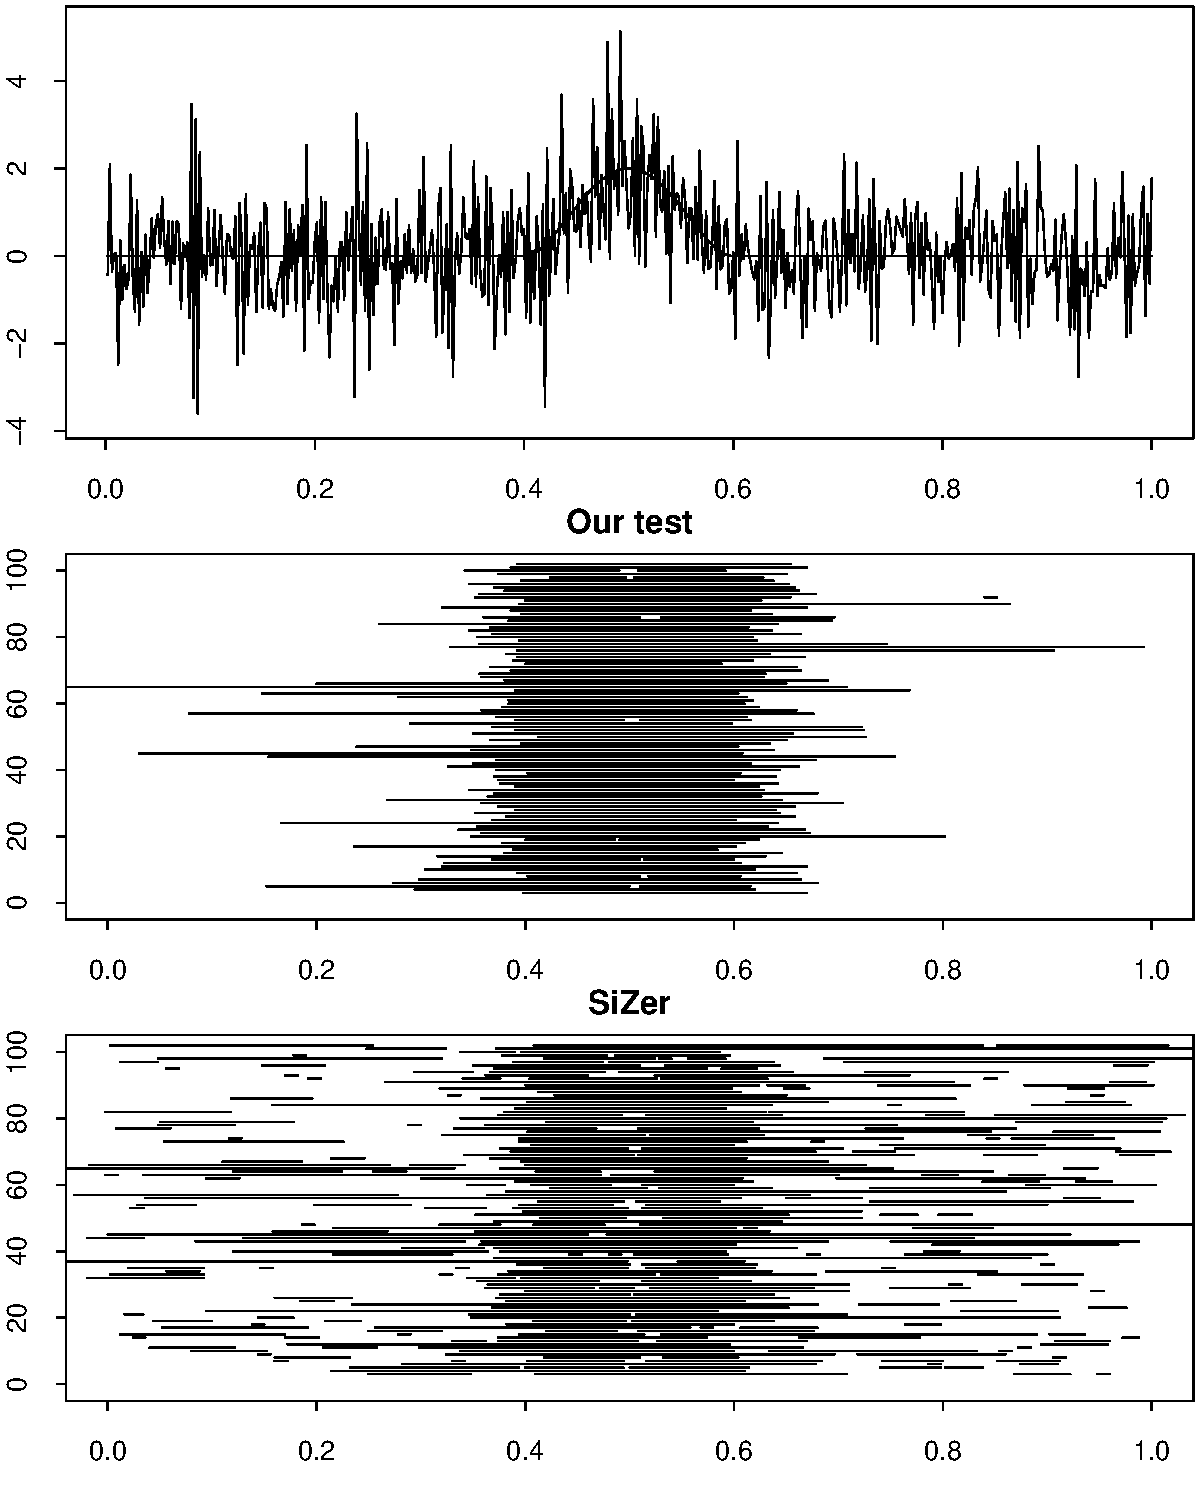
\includegraphics[width=.9\linewidth]{Plots/min_int_with_T_500_a1_-50.pdf}
\caption{$a_1 = -0.5$}
\end{subfigure}
\begin{subfigure}{.5\textwidth}
\centering
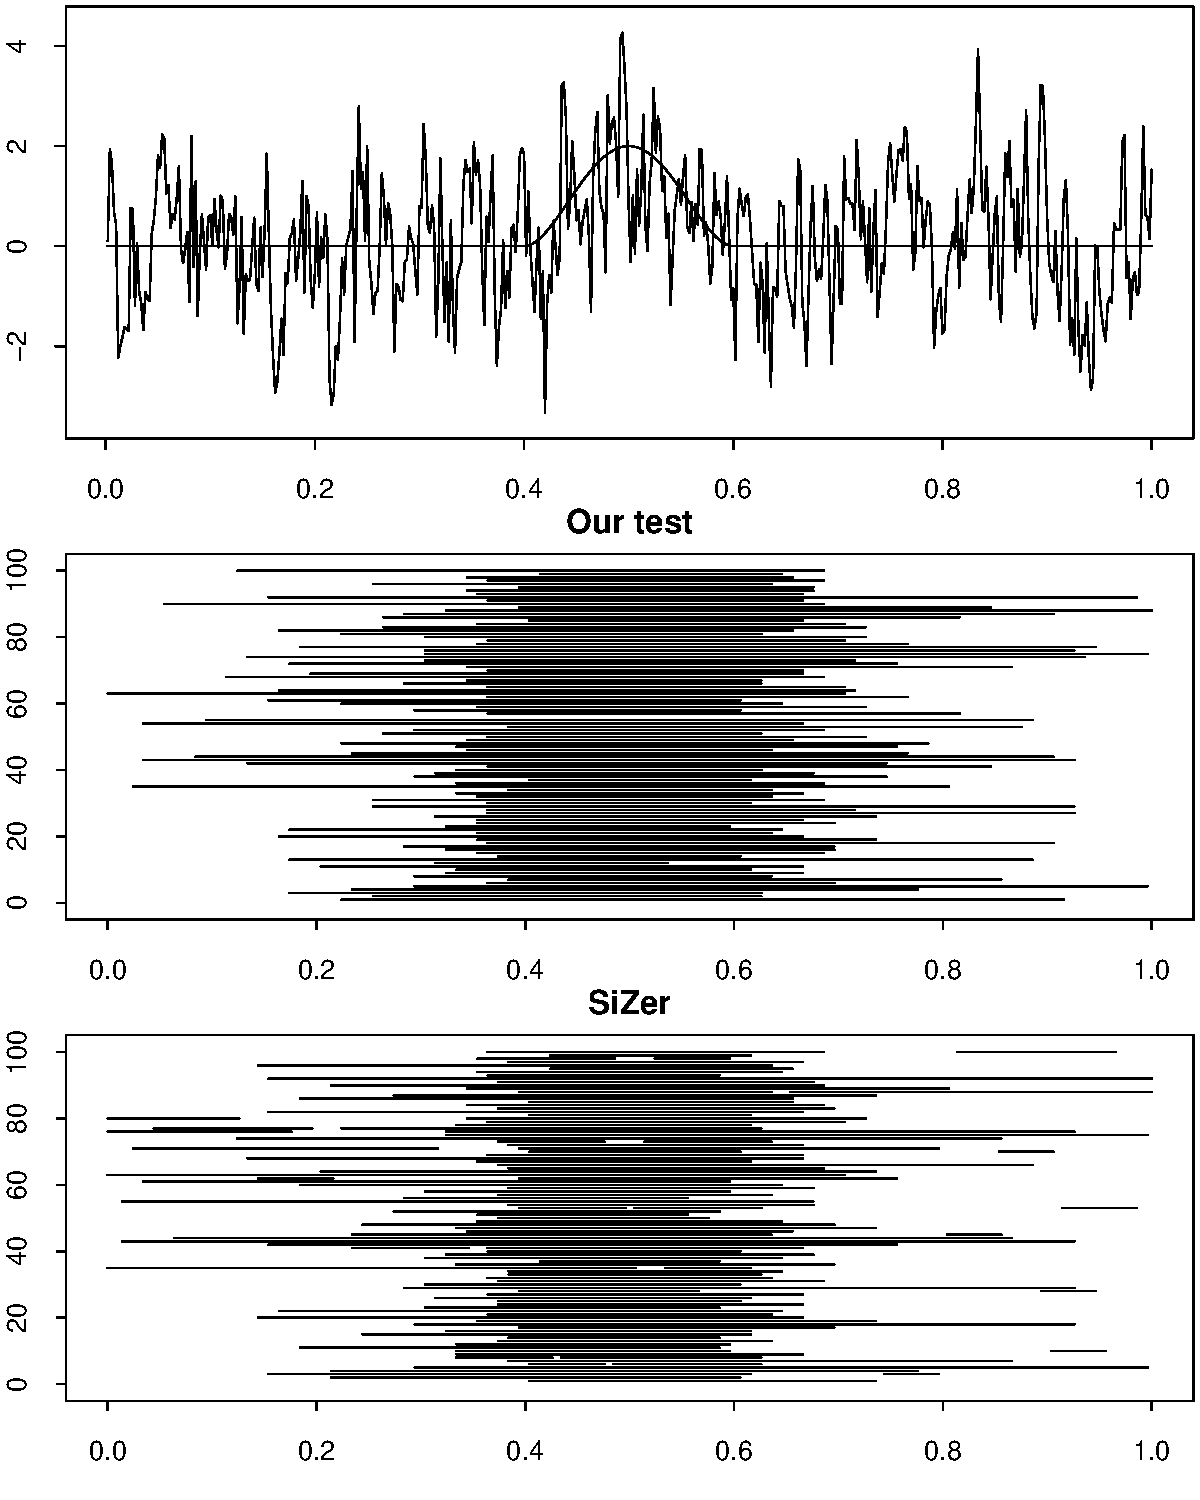
\includegraphics[width=.9\linewidth]{Plots/min_int_with_T_500_a1_50.pdf}
\caption{$a_1 = 0.5$}
\end{subfigure}
\caption{Comparison of the regions $\mathcal{R}_T^\pm$ and $\mathcal{R}_T^{\text{SiZer}}$. Subfigure (a) corresponds to the model setting with the AR parameter $a_1 = -0.5$, subfigure (b) to the setting with $a_1 = 0.5$. The upper panel of each subfigure shows a simulated time series path together with the underlying trend function $m$. The middle panel depicts the regions $\mathcal{R}_T^\pm$ produced by our multiscale test for $100$ simulation runs. The lower panel presents the regions $\mathcal{R}_T^{\text{SiZer}}$ produced by SiZer.}  
\label{fig:comparison_SiZer}
\end{figure}


We consider the same simulation setup as in the first part of the study, only the trend function $m$ is different. We let $m$ be defined as $m(u) = 2 \cdot \ind(u \in [0.4,0.6]) \cdot (1 - 100 \{u-0.5\}^2)^2$, which implies that $\mathcal{R} = [0.4,0.5) \cup (0.5,0.6]$. The function $m$ is plotted in the two upper panels of Figure \ref{fig:comparison_SiZer}. We set the significance level to $\alpha= 0.05$ and the sample size to $T=500$. For each AR parameter $a_1 \in \{ -0.5,0.5 \}$, we simulate $S=100$ samples and compute $\mathcal{R}_T^\pm$ and $\mathcal{R}_T^{\text{SiZer}}$ for each sample. The simulation results are depicted in Figure \ref{fig:comparison_SiZer}, the two subfigures (a) and (b) corresponding to different AR parameters. The upper panel of each subfigure displays the time series path of a representative simulation together with the trend function $m$. The middle panel shows the regions $\mathcal{R}_T^\pm$ produced by our multiscale approach for the $100$ simulation runs: On the $y$-axis, the simulation runs $i$ are enumerated for $1 \le i \le 100$, and the black line at $y$-level $i$ represents $\mathcal{R}_T^\pm$ for the $i$-th simulation. Finally, the lower panel of each subfigure depicts the regions $\mathcal{R}_T^{\text{SiZer}}$ in an analogous way. 


Inspecting Figure \ref{fig:comparison_SiZer}, our multiscale method can be seen to approximate the region $\mathcal{R}$ fairly well in both simulation scenarios under consideration. Especially for the negative AR parameter $a_1 = -0.5$, it performs substantially better than SiZer: For most simulations, $\mathcal{R}_T^\pm$ gives a good approximation to the region $\mathcal{R}$, whereas SiZer identifies regions of decrease/increase all over the unit interval $[0, 1]$. SiZer thus frequently mistakes fluctuations in the time series which are due to the dependence in the error terms for increases/decreases in $m$. For the positive AR parameter $a_1 = 0.5$, the difference in performance is not so pronounced. Nevertheless, also here, SiZer appears to spuriously detect increases/decreases in $m$ outside $\mathcal{R}$ more often than our method. 


To sum up, our multiscale test exhibits good size and power properties in the simulations, and the minimal intervals produced by it identify the time regions where $m$ increases/decreases in a quite reliable way. SiZer performs considerably worse in these respects. Nevertheless, it may still produce informative SiZer plots. % (which is what it is designed for anyway). 
All in all, we would like to regard the two methods as complementary rather than direct competitors. SiZer is an explorative tool which aims to give an overview of the increases/decreases in $m$ by means of a SiZer plot. Our method, in contrast, is tailored to be a rigorous statistical test of the hypothesis $H_0$. In particular, it allows to make rigorous confidence statements about the time regions where the trend $m$ increases/decreases. Such statements are not possible with SiZer. 


\subsection{Small sample properties of the long-run variance estimator}\label{subsec-sim-3}


In the final part of the simulation study, we examine the estimators of the AR parameters and the long-run error variance from Section \ref{subsec-error-var-AR}. We simulate data from the model $Y_{t,T} = m(t/T) + \varepsilon_t$, where $\{ \varepsilon_t\}$ is an AR($1$) process of the form $\varepsilon_t = a_1 \varepsilon_{t-1} + \eta_t$. We consider the AR parameters $a_1 \in \{-0.95,-0.75,-0.5,-0.25,0.25,0.5,0.75,0.95\}$, the sample sizze $T \in \{250, 500\}$ and let $\eta_t$ be i.i.d.\ standard normal innovation terms. For simplicity, $m$ is chosen to be a linear function of the form $m(u) = \beta u$ with the slope parameter $\beta$. For each value of $a_1$, we consider two different slopes $\beta$, one corresponding to a moderate and one to a pronounced trend $m$. 
%In particular, we let $\beta = s_\beta \cdot \sigma$ with $s_\beta = 1$ (moderate trend) and $s_\beta= 10$ (pronounced trend), where $\sigma^2$ is the long-run error variance.
In particular, we let $\beta = s_\beta \sqrt{\var(\varepsilon_t)}$ with $s_\beta \in \{1,10\}$. When $s_\beta = 1$, the slope $\beta$ is equal to the standard deviation $\sqrt{\var(\varepsilon_t)}$ of the error process, which yields a moderate trend $m$. When $s_\beta = 10$, in contrast, the slope $\beta$ is $10$ times as large as $\sqrt{\var(\varepsilon_t)}$, which results in a quite pronounced trend $m$. 

\begin{figure}[t!]
\begin{subfigure}[b]{0.475\textwidth}
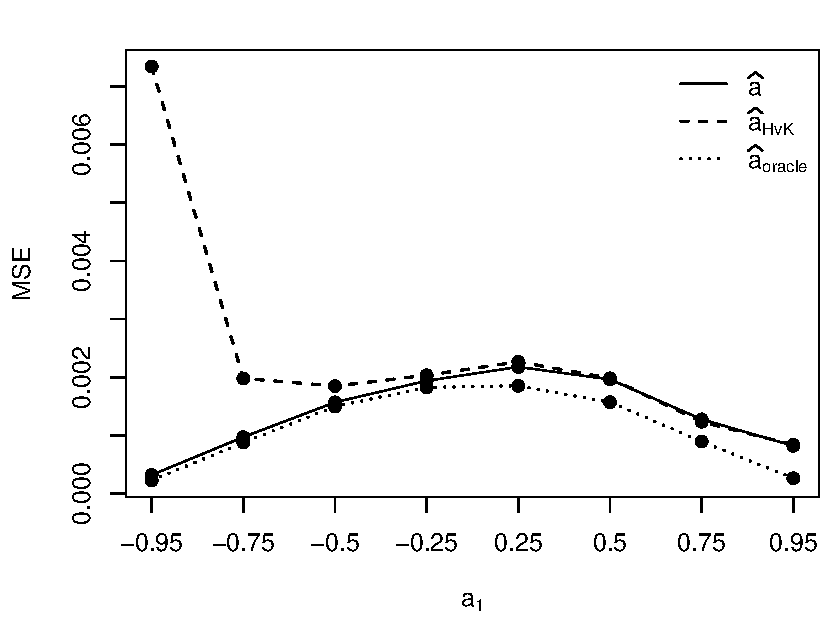
\includegraphics[width=\textwidth]{Plots/MSE_a1_T=500_slope=1_(q,K1,K2,M1,M2)=(25,2,10,20,30).pdf}
\end{subfigure}\hspace{0.25cm}
\begin{subfigure}[b]{0.475\textwidth}
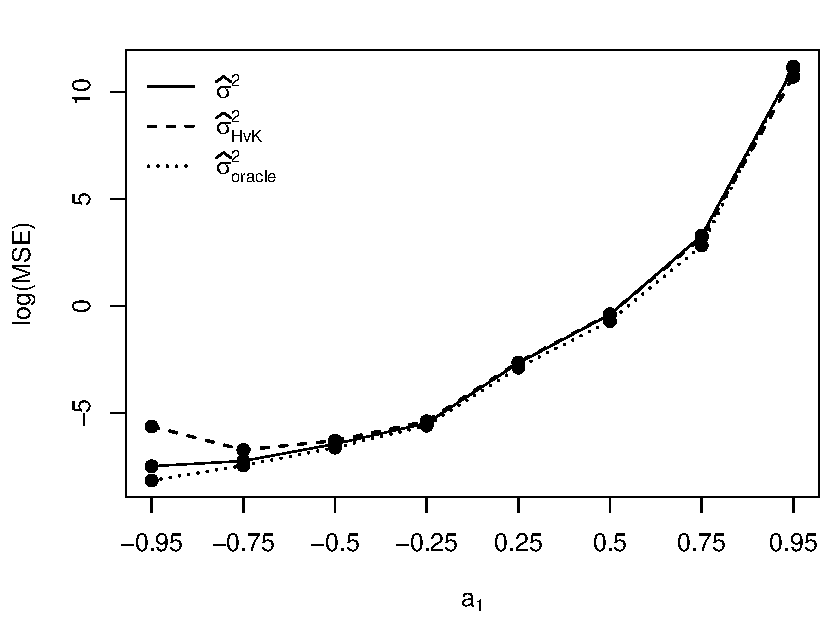
\includegraphics[width=\textwidth]{Plots/MSE_lrv_T=500_slope=1_(q,K1,K2,M1,M2)=(25,2,10,20,30).pdf}
\end{subfigure}
\caption{MSE values for the estimators $\widehat{a}$, $\widehat{a}_{\text{HvK}}$, $\widehat{a}_{\text{oracle}}$ and $\widehat{\sigma}^2$, $\widehat{\sigma}^2_{\text{HvK}}$ and $\widehat{\sigma}^2_{\text{oracle}}$ in the simulation scenarios with a moderate trend ($s_\beta=1$).}\label{fig:MSE_slope1}
\end{figure}

\begin{figure}[t!]
\begin{subfigure}[b]{0.475\textwidth}
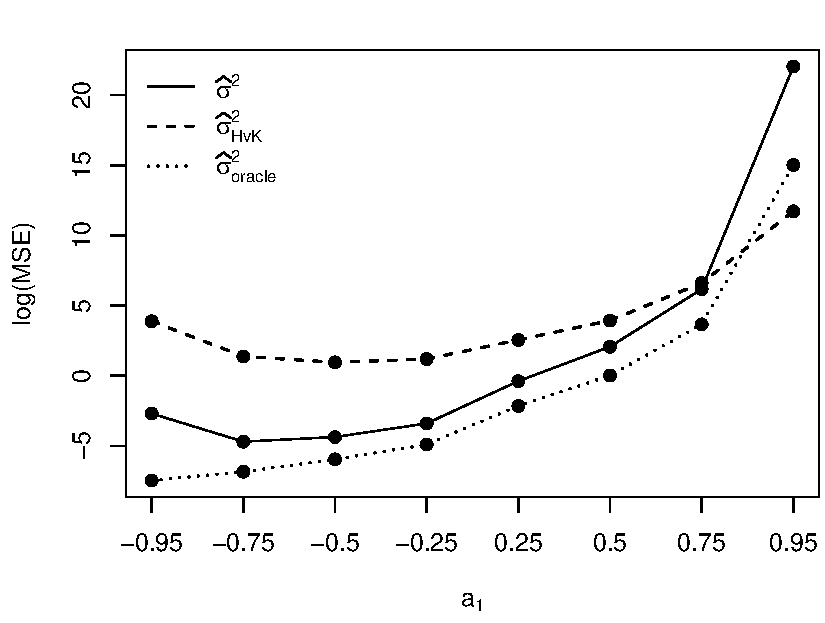
\includegraphics[width=\textwidth]{Plots/MSE_lrv_T=250_slope=10_(q,K1,K2,M1,M2)=(25,2,10,20,30).pdf}
\end{subfigure}\hspace{0.25cm}
\begin{subfigure}[b]{0.475\textwidth}
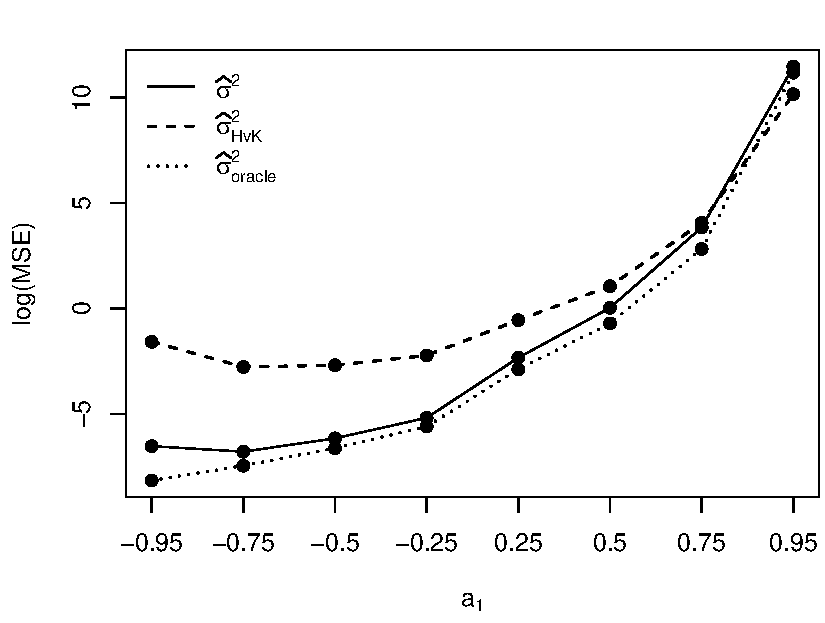
\includegraphics[width=\textwidth]{Plots/MSE_lrv_T=500_slope=10_(q,K1,K2,M1,M2)=(25,2,10,20,30).pdf}
\end{subfigure}
\caption{MSE values for the estimators $\widehat{a}$, $\widehat{a}_{\text{HvK}}$, $\widehat{a}_{\text{oracle}}$ and $\widehat{\sigma}^2$, $\widehat{\sigma}^2_{\text{HvK}}$, $\widehat{\sigma}^2_{\text{oracle}}$ in the simulation scenarios with a pronounced trend ($s_\beta=10$).}\label{fig:MSE_slope10}
\end{figure}


\begin{figure}[t!]
\centering
\begin{subfigure}[b]{\textwidth}
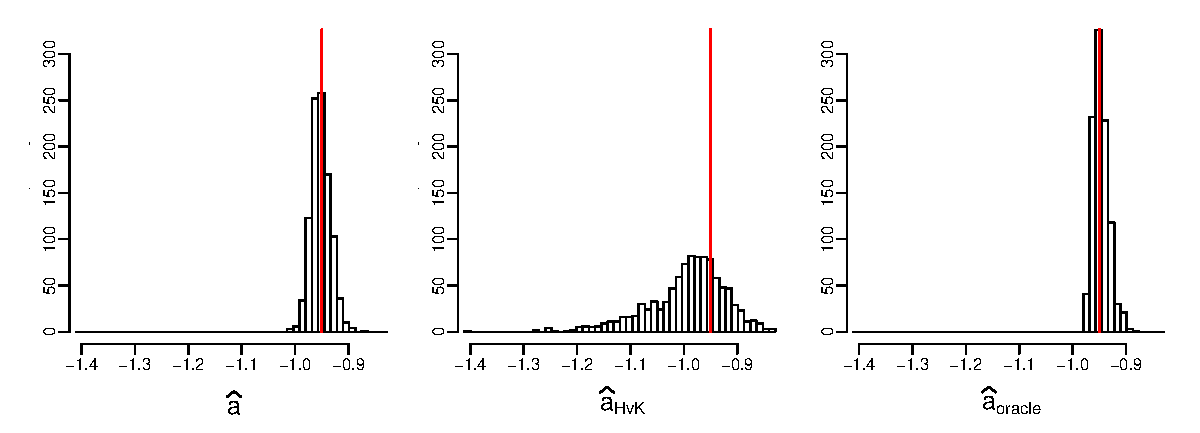
\includegraphics[width=\textwidth]{Plots/a_hat_histograms_a1=-95_T=500_slope=1_(q,K1,K2,M1,M2)=(25,2,10,20,30).pdf}
\end{subfigure}
\begin{subfigure}[b]{\textwidth}
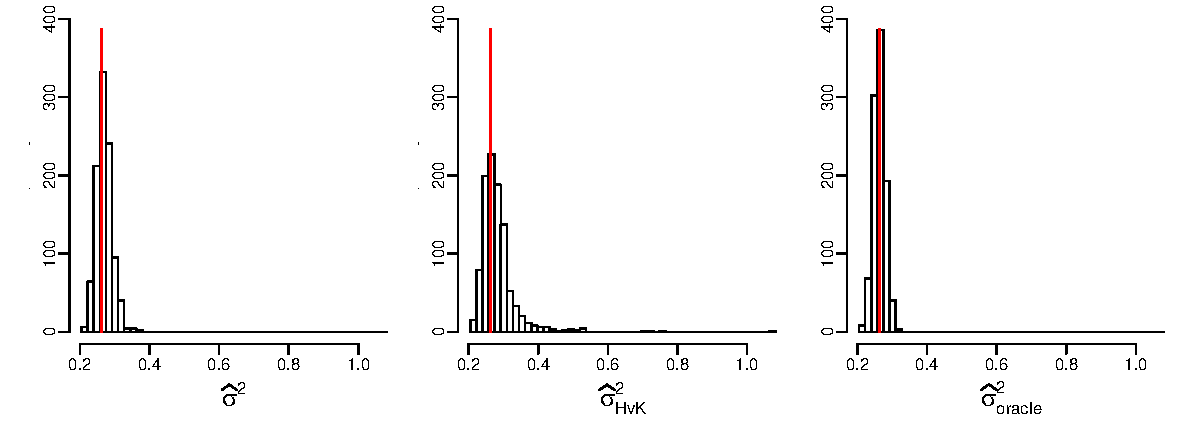
\includegraphics[width=\textwidth]{Plots/lrv_histograms_a1=-95_T=500_slope=1_(q,K1,K2,M1,M2)=(25,2,10,20,30).pdf}
\end{subfigure}
\caption{Histograms of the simulated values produced by the estimators $\widehat{a}$, $\widehat{a}_{\text{HvK}}$, $\widehat{a}_{\text{oracle}}$, $\widehat{\sigma}^2$, $\widehat{\sigma}^2_{\text{HvK}}$, $\widehat{\sigma}^2_{\text{oracle}}$ in the scenario with $T=500$, $a_1 = -0.95$ and $\beta = 1$. The vertical red lines indicate the true values of $a_1$ and $\sigma^2$.}\label{fig:hist_scenario1} 
\end{figure}


\begin{figure}[t!]
\centering
\begin{subfigure}[b]{\textwidth}
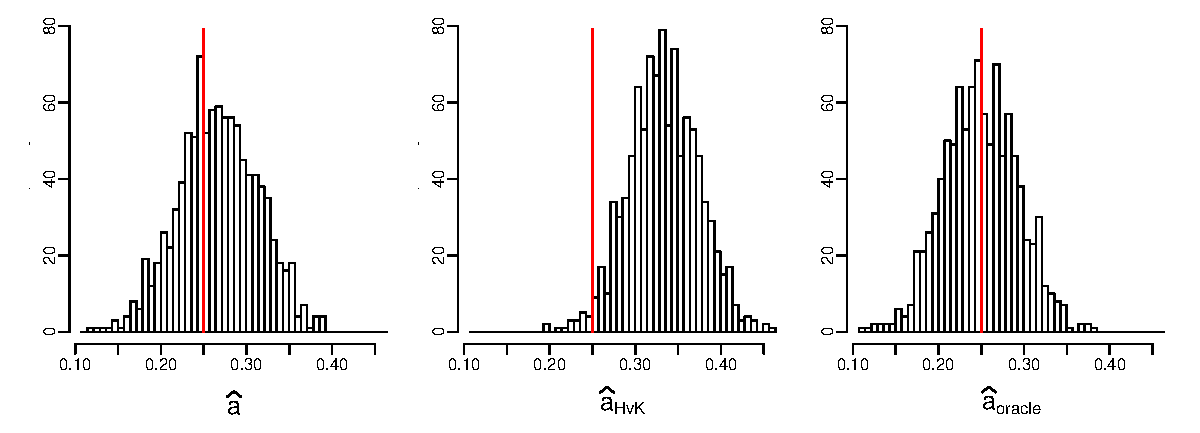
\includegraphics[width=\textwidth]{Plots/a_hat_histograms_a1=25_T=500_slope=10_(q,K1,K2,M1,M2)=(25,2,10,20,30).pdf}
\end{subfigure}
\begin{subfigure}[b]{\textwidth}
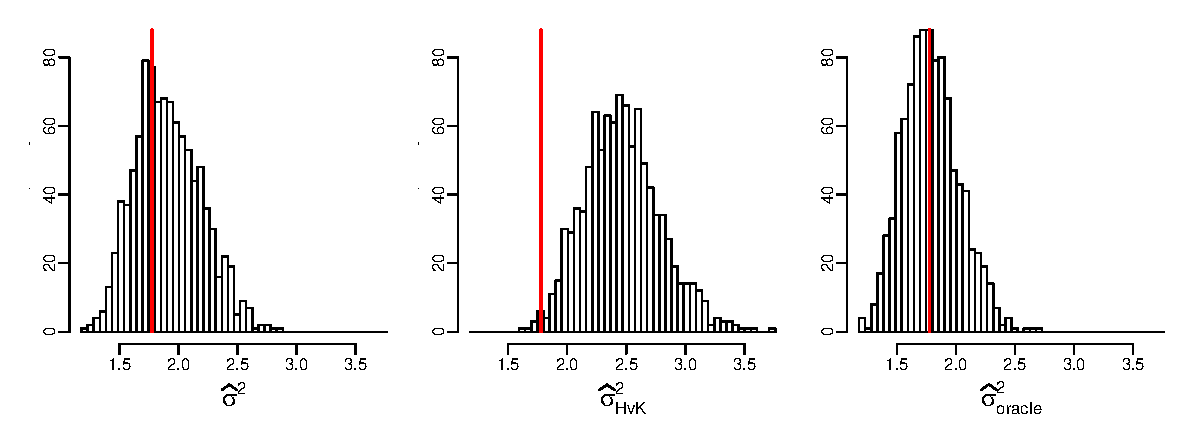
\includegraphics[width=\textwidth]{Plots/lrv_histograms_a1=25_T=500_slope=10_(q,K1,K2,M1,M2)=(25,2,10,20,30).pdf}
\end{subfigure}
\caption{Histograms of the simulated values produced by the estimators $\widehat{a}$, $\widehat{a}_{\text{HvK}}$, $\widehat{a}_{\text{oracle}}$ and $\widehat{\sigma}^2$, $\widehat{\sigma}^2_{\text{HvK}}$, $\widehat{\sigma}^2_{\text{oracle}}$ in the scenario with $T=500$, $a_1 = 0.25$ and $\beta = 10$. The vertical red lines indicate the true values of $a_1$ and $\sigma^2$.}\label{fig:hist_scenario2} 
\end{figure}


For each model specification, we generate $S=1000$ data samples and compute the following quantities for each simulated sample: 
\begin{enumerate}[label=(\roman*),leftmargin=0.9cm]
\item the pilot estimator $\widetilde{a}_q$ from \eqref{est-AR-FS} with the tuning parameter $q$.
\item the estimator $\widehat{a}$ from \eqref{est-AR} with the tuning parameter $\overline{r} = r$ as well as the long-run variance estimator $\widehat{\sigma}^2$ from \eqref{est-lrv}. 
\item the estimators of $a$ and $\sigma^2$ from \cite{Hall2003}, which are denoted by $\widehat{a}_{\text{HvK}}$ and $\widehat{\sigma}^2_{\text{HvK}}$ for ease of reference. The estimator $\widehat{a}_{\text{HvK}}$ is computed as described in Section 2.2 of \cite{Hall2003} and $\widehat{\sigma}^2_{\text{HvK}}$ as defined at the bottom of p.447 in Section 2.3. The estimator $\widehat{a}_{\text{HvK}}$ (as well as $\widehat{\sigma}^2_{\text{HvK}}$) depends on two tuning parameters which we denote by $m_1$ and $m_2$ as in \cite{Hall2003}. 
\item oracle estimators $\widehat{a}_{\text{oracle}}$ and $\widehat{\sigma}^2_{\text{oracle}}$ of $a_1$ and $\sigma^2$, which are constructed under the assumption that the error process $\{\varepsilon_t\}$ is observed. For each simulation run, we compute $\widehat{a}_{\text{oracle}}$ as the maximum likelihood estimator of $a_1$ from the time series of simulated error terms $\varepsilon_1,\ldots,\varepsilon_T$. We then calculate the residuals $r_t = \varepsilon_t - \widehat{a}_{\text{oracle}} \, \varepsilon_{t-1}$ and estimate the innovation variance $\nu^2 = \ex[\eta_t^2]$ by $\widehat{\nu}_{\text{oracle}}^2 = (T-1)^{-1} \sum_{t=2}^T r_t^2$. Finally, we set $\widehat{\sigma}^2_{\text{oracle}} = \widehat{\nu}_{\text{oracle}}^2 / (1 - \widehat{a}_{\text{oracle}})^2$. 
\end{enumerate}
Throughout the section, we set $q = 25$, $\underline{r} = p + 1$, where $p = 1$ is the order, $\overline{r} = r = 10$ and $(m_1,m_2) = (20,30)$. We in particular choose $q$ to be in the middle of $m_1$ and $m_2$ to make the tuning parameters of the estimators $\widetilde{a}_q$ and $\widehat{a}_{\text{HvK}}$ more or less comparable. In order to assess how sensitive our estimators are to the choice of $q$ and $r$, we carry out a number of robustness checks, considering a range of different values for $q$ and $r$. In addition, we vary the tuning parameters $m_1$ and $m_2$ of the estimators from \cite{Hall2003} in order to make sure that the results of our comparison study are not driven by the particular choice of any of the involved tuning parameters. The results of our robustness checks are reported in Section S.3 of the Supplementary Material. They show that the results of our comparison study are robust to %persist across 
different choices of the parameters $q$, $r$ and $(m_1,m_2)$. Moreover, they indicate that our estimators are rather insensitive to the choice of tuning parameters. 


For each estimator $\widehat{a}$, $\widehat{a}_{\text{HvK}}$, $\widehat{a}_{\text{oracle}}$ and $\widehat{\sigma}^2$, $\widehat{\sigma}^2_{\text{HvK}}$, $\widehat{\sigma}^2_{\text{oracle}}$ and for each model specification, the simulation output consists in a vector of length $S=1000$ which contains the $1000$ simulated values of the respective estimator. Figures \ref{fig:MSE_slope1} and \ref{fig:MSE_slope10} report the mean squared error (MSE) of the estimators computed from these $1000$ values. The different plots in the two figures correspond to different simulation scenarios. On the $x$-axis of each plot, the various values of the AR parameter $a_1$ are listed which are considered. The solid line in each plot gives the MSE values of our estimators. The dashed and dotted lines specify the MSE values of the HvK and the oracle estimators, respectively. Note that for the long-run variance estimators, the plots report the logarithm of the MSE rather than the MSE itself since the MSE values are too different across simulation scenarios to obtain a reasonable graphic presentation. In addition to the MSE values presented in Figures \ref{fig:MSE_slope1} and \ref{fig:MSE_slope10}, we depict histograms of the $1000$ simulated values produced by the estimators $\widehat{a}$, $\widehat{a}_{\text{HvK}}$, $\widehat{a}_{\text{oracle}}$ and $\widehat{\sigma}^2$, $\widehat{\sigma}^2_{\text{HvK}}$, $\widehat{\sigma}^2_{\text{oracle}}$ for two specific simulation scenarios in Figures \ref{fig:hist_scenario1} and \ref{fig:hist_scenario2}. The main findings can be summarized as follows:  
\begin{enumerate}[label=(\roman*),leftmargin=0.9cm]

%\item The performance of our second-step estimators $\widehat{a}$ and $\widehat{\sigma}^2$ is fairly close to that of the oracle estimators $\widehat{a}_{\text{oracle}}$ and $\widehat{\sigma}^2_{\text{oracle}}$ in all of the considered simulation scenarios. In particular, the mean values and standard deviations in Tables \ref{tab:AR_parameters} and \ref{tab:lrv} are quite similar for our estimators and the corresponding oracles. 

\item In the simulation scenarios with a moderate trend ($\beta = 1$), the estimators $\widehat{a}_{\text{HvK}}$ and $\widehat{\sigma}^2_{\text{HvK}}$ of \cite{Hall2003} exhibit a similar performance as our estimators $\widehat{a}$ and $\widehat{\sigma}^2$ as long as the AR parameter $a_1$ is not too close to $-1$. For strongly negative values of $a_1$ (in particular for $a_1 = -0.75$ and $a_1 = -0.95$), the estimators perform much worse than ours. This can be clearly seen from the much larger MSE values of the estimators  $\widehat{a}_{\text{HvK}}$ and $\widehat{\sigma}^2_{\text{HvK}}$ for $a_1 = -0.75$ and $a_1 = -0.95$ in Figure \ref{fig:MSE_slope1}. Figure \ref{fig:hist_scenario1} gives some further insights into what is happening here. It shows the histograms of the simulated values produced by the estimators $\widehat{a}$, $\widehat{a}_{\text{HvK}}$, $\widehat{a}_{\text{oracle}}$ and the corresponding long-run variance estimators in the scenario with $T=500$, $a_1=-0.95$ and $\beta = 1$. As can be seen, the estimator $\widehat{a}_{\text{HvK}}$ does not obey the causality restriction $|a_1| \le 1$ but frequently takes values substantially smaller than $-1$. This results in a very large spread of the histogram and thus in a disastrous performance of the estimator.\footnote{One could of course set $\widehat{a}_{\text{HvK}}$ to $-(1 - \delta)$ for some small $\delta > 0$ whenever it takes a value smaller than $-1$. This modified estimator, however, is still far from performing in a satisfying way when $a_1$ is close to $-1$.} A similar point applies to the histogram of the long-run variance estimator $\widehat{\sigma}^2_{\text{HvK}}$. Our estimators $\widehat{a}$ and $\widehat{\sigma}^2$, in contrast, exhibit a stable behaviour in this case. \\ %An analogous point applies to the long-run variance estimators $\widehat{\sigma}^2$ and $\widehat{\sigma}^2_{\text{HvK}}$. 
Interestingly, the estimator $\widehat{a}_{\text{HvK}}$ (as well as the corresponding long-run variance estimator $\widehat{\sigma}^2_{\text{HvK}}$) performs much worse than ours for large negative values but not for large positive values of $a_1$. This can be explained as follows: In the special case of an AR($1$) process, the estimator $\widehat{a}_{\text{HvK}}$ may produce estimates smaller than $-1$ but it cannot become larger than $1$. This can be easily seen upon inspecting the definition of the estimator. Hence, for large positive values of $a_1$, the estimator $\widehat{a}_{\text{HvK}}$ performs well as it satisfies the causality restriction that the estimated AR parameter should be smaller than $1$. 

\item In the simulation scenarios with a pronounced trend ($\beta = 10$), the estimators of \cite{Hall2003} perform much worse than ours for most of the AR parameters $a_1$ under consideration. In particular, their MSE values reported in Figure \ref{fig:MSE_slope10} are much larger than the values produced by our estimators for most values of $a_1$. The reason is the following: The estimators have a strong bias since the pronounced trend with $\beta = 10$ is not eliminated appropriately by the underlying differencing methods. This point is nicely illustrated by Figure \ref{fig:hist_scenario2} which shows histograms of the simulated values of the estimators $\widehat{a}$, $\widehat{a}_{\text{HvK}}$, $\widehat{a}_{\text{oracle}}$ and the corresponding long-run variance estimators in the scenario with $T=500$, $a_1=0.25$ and $\beta = 10$. As can be seen, the histogram produced by our estimator $\widehat{a}$ is centred around the true value $a_1 = 0.25$, whereas that of the estimator $\widehat{a}_{\text{HvK}}$ is strongly biased upwards. A similar picture arises for the long-run variance estimators $\widehat{\sigma}^2$ and $\widehat{\sigma}^2_{\text{HvK}}$. \\
Whereas the methods of \cite{Hall2003} perform much worse than ours for negative and moderately positive values of $a_1$, the performance is fairly similar for large values of $a_1$. In particular, the MSE values produced by the estimators of \cite{Hall2003} and ours are much closer for large positive values of $a_1$. This can be explained as follows: When the trend $m$ is not eliminated appropriately by taking differences, this creates spurious persistence in the data. Hence, the estimator $\widehat{a}_{\text{HvK}}$ tends to overestimate the AR parameter $a_1$, that is, $\widehat{a}_{\text{HvK}}$ tends to be larger in absolute value than $a_1$. Very loosely speaking, when the parameter $a_1$ is close to $1$, say $a_1 = 0.95$, there is not much room for overestimation since $\widehat{a}_{\text{HvK}}$ cannot become larger than $1$. Consequently, the effect of not eliminating the trend appropriately has a much smaller effect on $\widehat{a}_{\text{HvK}}$ for large positive values of $a_1$. 

%\item In all of the simulation scenarios under consideration, in particular both when the trend is moderate ($\beta = 1$) and pronounced ($\beta = 10$), the MSE values produced by our estimators are fairly close to those of the oracle estimators as can be seen by inspecting Figures \ref{fig:MSE_slope1} and \ref{fig:MSE_slope10}. Only  

\end{enumerate}



\section{Application}\label{sec-data}


The analysis of time trends in long temperature records is an important task in climatology. Information on the shape of the trend is needed in order to better understand long-term climate variability. The Central England temperature record is the longest instrumental temperature time series in the world. It is a valuable asset for analysing climate variability over the last few hundred years. The data is publicly available on the webpage of the UK Met Office. A detailed description of the data can be found in \cite{Parker1992}. For our analysis, we use the dataset of yearly mean temperatures which consists of $T=359$ observations covering the years from $1659$ to $2017$. We assume that the data follow the nonparametric trend model $Y_{t,T} = m(t/T) + \varepsilon_t$, where $m$ is the unknown time trend of interest. The error process $\{ \varepsilon_t \}$ is supposed to have the AR($p$) structure $\varepsilon_t = \sum_{j=1}^p a_j \varepsilon_{t-j} + \eta_t$, where $\eta_t$ are i.i.d.\ innovations with mean $0$ and variance $\nu^2$. As pointed out in \cite{Mudelsee2010} among others, this is the most widely used error model for discrete climate time series. To select the AR order $p$, we proceed as follows: We estimate the AR parameters and the corresponding variance of the innovation terms for different AR orders by our methods from Section \ref{subsec-error-var-AR} and choose $p$ to be the minimizer of the final prediction error (FPE) criterion. This yields the AR order $p = 2$. We then estimate the parameters $\boldsymbol{a} = (a_1,a_2)$ and the long error run-variance $\sigma^2$ by the estimators $\widehat{\boldsymbol{a}} = (\widehat{a}_1,\widehat{a}_2)$ and $\widehat{\sigma}^2$, where we set $q = 20$ and $(\underline{r},\overline{r}) = (5,10)$ as in the simulation study of Section \ref{subsec-sim-1}. We thus obtain the estimates $\widehat{a}_1 \approx ??$, $\widehat{a}_2 \approx ??$ and $\widehat{\sigma}^2 \approx ??$.


\begin{figure}[t]
\centering
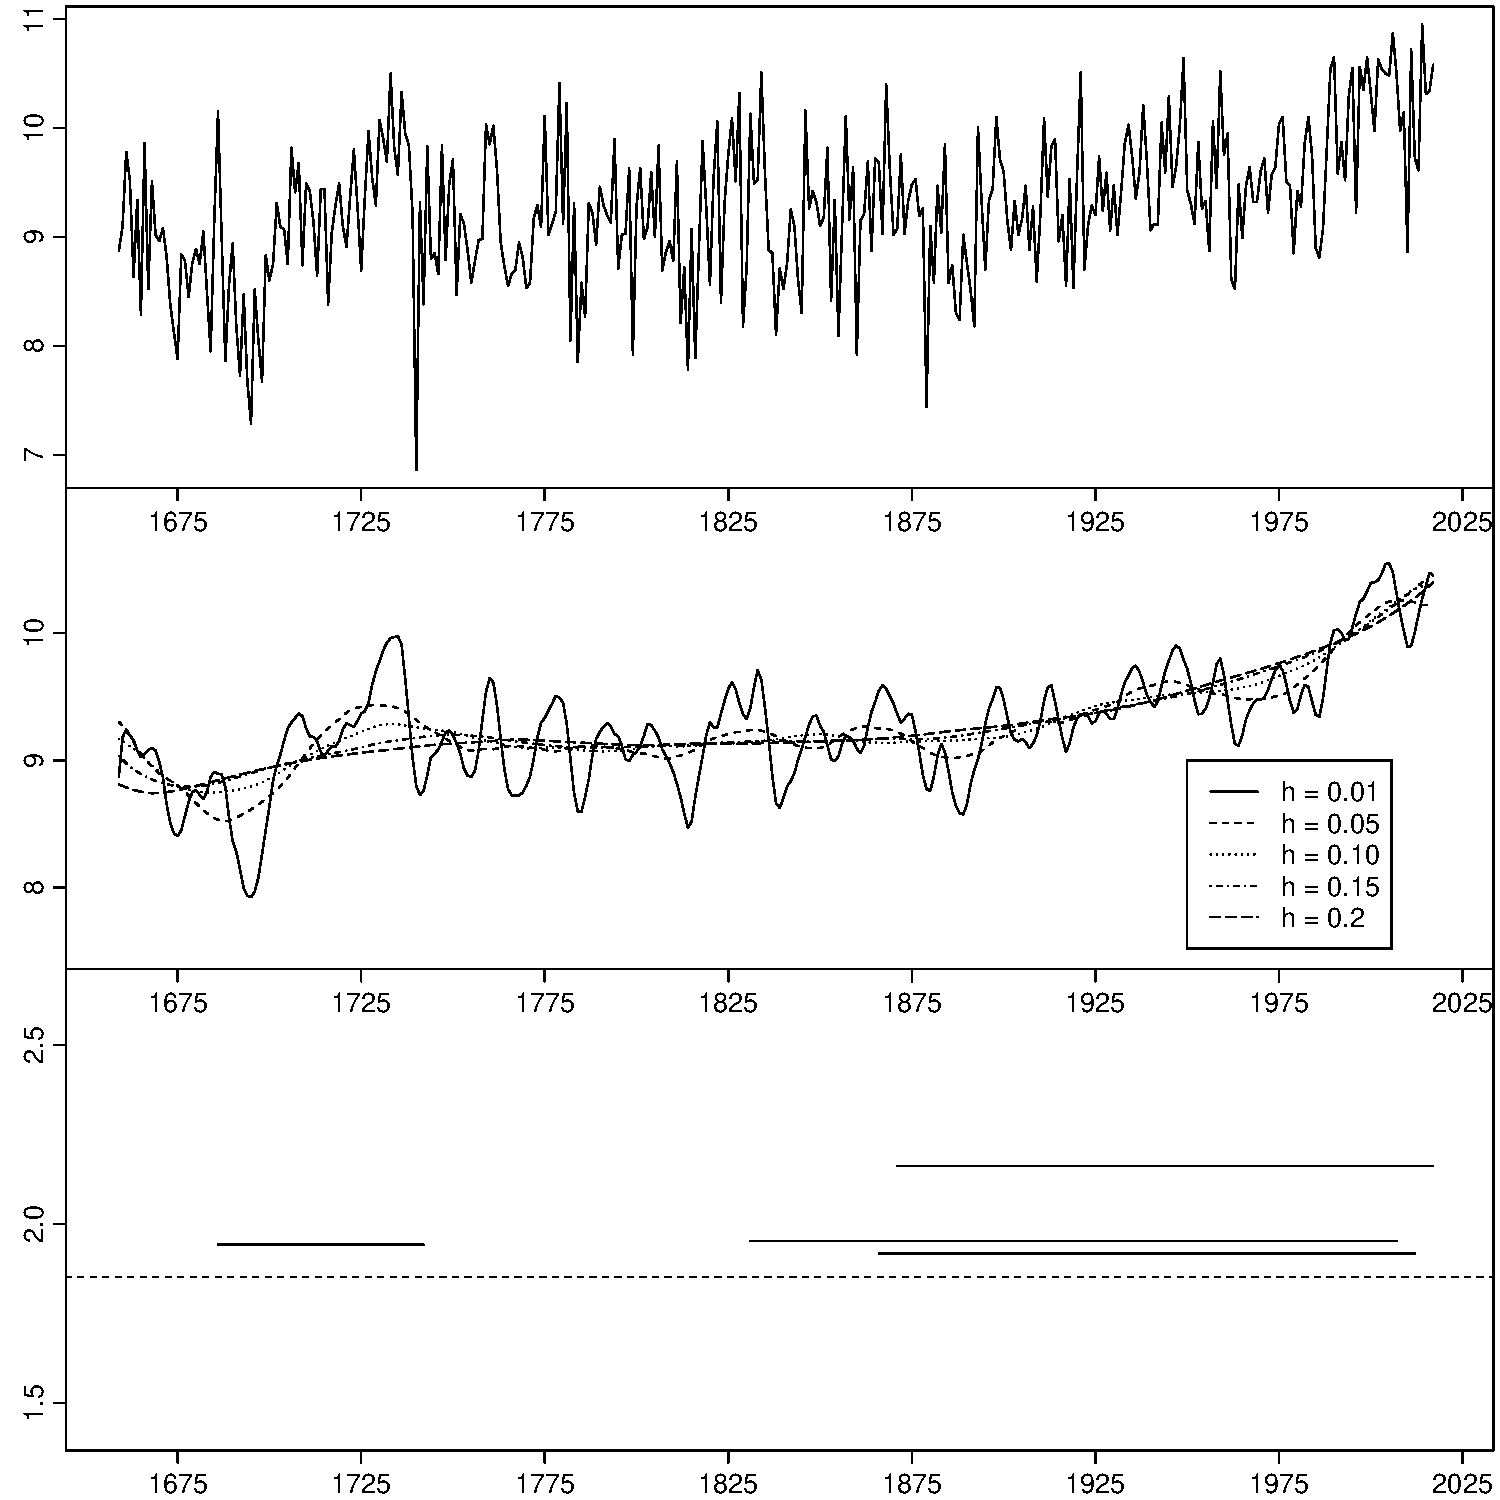
\includegraphics[width=0.8\textwidth]{Plots/temperature_L1_20_L2_30.pdf}
\caption{Summary of the application results for Section \ref{sec-data}. The upper panel shows the Central England mean temperature time series. The middle panel depicts local linear kernel estimates of the time trend for a number of different bandwidths $h$. The lower panel presents the minimal intervals in the set $\Pi_T^+$ produced by the multiscale test. These are $[??,??]$, $[??,??]$, $[??,??]$ and $[??,??]$.}\label{plot-results-app1}
\end{figure}


With the help of our multiscale method from Section \ref{sec-method}, we test the null hypothesis $H_0$ that $m$ is constant on all intervals $[u-h,u+h]$ with $(u,h) \in \mathcal{G}_T$, where we use the grid $\mathcal{G}_T$ defined in \eqref{grid-sim-app}. To do so, we set the significance level to $\alpha = 0.05$ and implement the test in exactly the same way as in the simulations of Section \ref{sec-sim}. The results are presented in Figure \ref{plot-results-app1}. The upper panel shows the raw temperature time series, whereas the middle panel depicts local linear kernel estimates of the trend $m$ for different bandwidths $h$. As one can see, the shape of the estimated time trend strongly differs with the chosen bandwidth. When the bandwidth is small, there are many local increases and decreases in the estimated trend. When the bandwidth is large, most of these local variations get smoothed out. Hence, by themselves, the nonparametric fits do not give much information on whether the trend $m$ is increasing or decreasing in certain time regions. 


Our multiscale test provides this kind of information, which is summarized in the lower panel of Figure \ref{plot-results-app1}. The plot depicts the minimal intervals contained in the set $\Pi_T^+$ which is defined in Section \ref{subsec-method-theo}. The set of intervals $\Pi_T^-$ is empty in the present case. The height at which a minimal interval $I_{u,h} = [u-h,u+h] \in \Pi_t^+$ is plotted indicates the value of the corresponding (additively corrected) test statistic $\widehat{\psi}_T(u,h) / \widehat{\sigma} - \lambda(h)$. The dashed line specifies the critical value $q_T(\alpha)$, where $\alpha = 0.05$ as already mentioned above. According to Proposition \ref{prop-test-3}, we can make the following simultaneous confidence statement about the collection of minimal intervals in $\Pi_T^+$. We can claim, with confidence of about $95\%$, that the trend function $m$ has some increase on each minimal interval. More specifically, we can claim with this confidence that there has been some upward movement in the trend both in the period from around $1680$ to $1740$ and in the period from about $1880$ onwards. Hence, our test in particular provides evidence that there has been some warming trend in the period over approximately the last $140$ years. On the other hand, as the set $\Pi_T^-$ is empty, there is no evidence of any downward movement of the trend.  

